
\chapter{Deep learning}
In this chapter we are going to introduce deep learning, methods of which are going to be implemented in our solution. We will introduce general principles and take a closer look on artificial neural networks, with main focus on convolutional neural networks. Lastly, the topic of interpretability and explainability of neural networks is discussed, with an emphasis on Layer-wise Relevance Propagation.

Deep learning is a form of machine learning, which is a significant part of the scientific field known as artificial intelligence. Over the past decade, a remarkable progress has been made in application of machine learning systems in numerous fields of science as well as in everyday life \cite{longsurvey2018}. They are used in natural language processing, detection of objects in images or speech recognition. These systems thrive mainly because of growing amounts of available data and empowerment of fast GPU computing, both of which is important for their proper training. The usage of machine learning in medicine benefits primarily from ascending volume of digitalized patient data. In 2017 in the United States alone, 150 exabytes of medical data was generated and this number increases annually by approximately 47\% \cite{stanford2017}. With that said, deep learning systems are able to move from theory to practice and assist physicians in hospitals and health centers. According to Stanford Medicine Health Trends Report of 2020 \cite{stanford2020} up to June 2019, the U.S. Food and Drug Administration had approved a total of 46 machine learning algorithms for medical purposes. As machine learning and its applications is still being explored, we can expect this number to further increase rapidly.

Deep learning enables computational models, which are composed of several processing layers, to learn representations of data, which contain multiple  underlying levels of abstraction \cite{greekDeepLearning}. It allows computers to learn from experience and comprehend the world more like a human - as a hierarchy, where complicated concepts are composed of more simple ones. \cite{deeplearningbook} The conventional machine learning approach required a human expert to do a hand-crafted engineering to extract features from data prior to feeding it to a machine, which required much more time and resources. The key advantage of deep learning is that the features are learned by the machine automatically, thanks to a data-driven approach throughout the learning process \cite{deeplearningHealthcare}. 



\section{Deep learning categorization}
We distinguish several primary forms of machine learning, which can be applied to deep learning as well. The main two, which we will discuss in our work, are supervised and unsupervised learning.  \cite{lecundeeplearning} These two forms differ mainly in whether labeled data, corresponding to the input data, is available for the training process. There is a form of learning known as semi-supervised, which we will, however, not further discuss.

\subsection{Supervised learning}
Supervised learning  is the most frequently used form of machine learning \cite{lecundeeplearning}. As it's name suggests, systems which fall under this category are trained under a certain form of supervision, which is present to guide the learning process. During training, a function is computed after each prediction, which measures the error rate of the model. According to the computed value, the internal parameters of the machine are adjusted in order to minimise the error rate in future predictions. These adjustable parameters are the model's most important component. A procedure which empowers nearly all deep learning models' error rate computation and ensures the parameter adjustment is called Stochastic gradient descent. We will discuss this procedure in more detail later in this chapter. Classification and regression are the two main tasks, which supervised learning attempts to solve \cite{kim2019deep}. Our solution will work with labeled data, thus it falls under the category of supervised learning.

\subsection{Unsupervised learning} The technique used by unsupervised learning algorithms is to learn important features contained in the training data without any supervision, as the name implies \cite{deeplearningbook}. Unsupervised learning model attempts to automatically discover the underlying information by extracting and analyzing useful features. This type of learning does not require the training data to be labeled with the correct answer. In this matter embodies it's biggest advantage - withdrawal from the need of labeled data, which would require manual intervention and is not always easy to obtain. Although there is no distinct line between supervised and unsupervised concepts, we can say that the most widely used unsupervised learning algorithms are clustering, principal components analysis, anomaly detection or generative adversarial networks \cite{deeplearningbook, kim2019deep}.

\section{Artificial neural networks}
This section is primarily dedicated to deep neural networks, which are the core of our solution. However, in order to gain better perspective, we will first introduce some conceptual and historical context of artificial neural networks in general.\\
Proposed in the 1940s, artificial neural network (ANN) is a computational model, which is a part of the broad artificial intelligence field. The word "neural" refers to the fact, that it was initially inspired by the way human brain functions. There are approximately $10^{11}$ neurons inside a human brain \cite{navrat2007umela}. Neuron is an elementary cell of the neural system, in which biochemical processes ensure the possibility of processing and sending neural signals. These signals are often referred to as activations. Neurons are interconnected by special joints called synopses, which enables them to communicate \cite{navrat2007umela}. Throughout the whole life, the importance and strength of synopses between neurons change, impacted by human's experience and learning. Artificial neural networks simulate the structure, as well as the behaviour of neurons. If we were to apply the biological terms to an ANN, synopses would be called weights
\subsection*{Perceptron} 
Perceptron is the earliest model of a neural network, composed of a single neuron. The output \textit{o} of the perceptron is defined by the following formula:
\begin{equation}
    o = f(net) = f(\bar w \cdot \bar x) = f (\sum_{j=1}^{n+1} w_jx_j)
\end{equation}
where $f$ is the activation function, $\bar w$ is the weights vector, $\bar x$ is a vector of the input signals. This perceptron calculates with having $n+1$ inputs \cite{navrat2007umela}. The abilities of a single perceptron are quite constrained. It only manages to classify input data into two separate classes. With that said, perceptron provides a solution only to linearly separable problems \cite{navrat2007umela}.
\subsection*{Feedforward neural networks}
Most real-world problems do not have linear character and can not be tackled with the simple perceptron model. A solution to this problem was introduced in 1980s when feedforward neural networks with the backpropagation algorithm were proposed \cite{navrat2007umela}. Multiple neurons (perceptrons) arranged in layers is what constructs a feedforward neural network. In this type of network, the information is passed only in the forward direction and the connections between neurons form a directed acyclic graph. In other words, each neuron from layer \textit{l} sends signals to each neuron in layer \textit{l+1}. The very first (leftmost) layer in a network is called input layer and the last (rightmost) is called output layer. In between, one middle layer, often also called "hidden" layer, is situated. 
\begin{figure}[!ht]
\centering
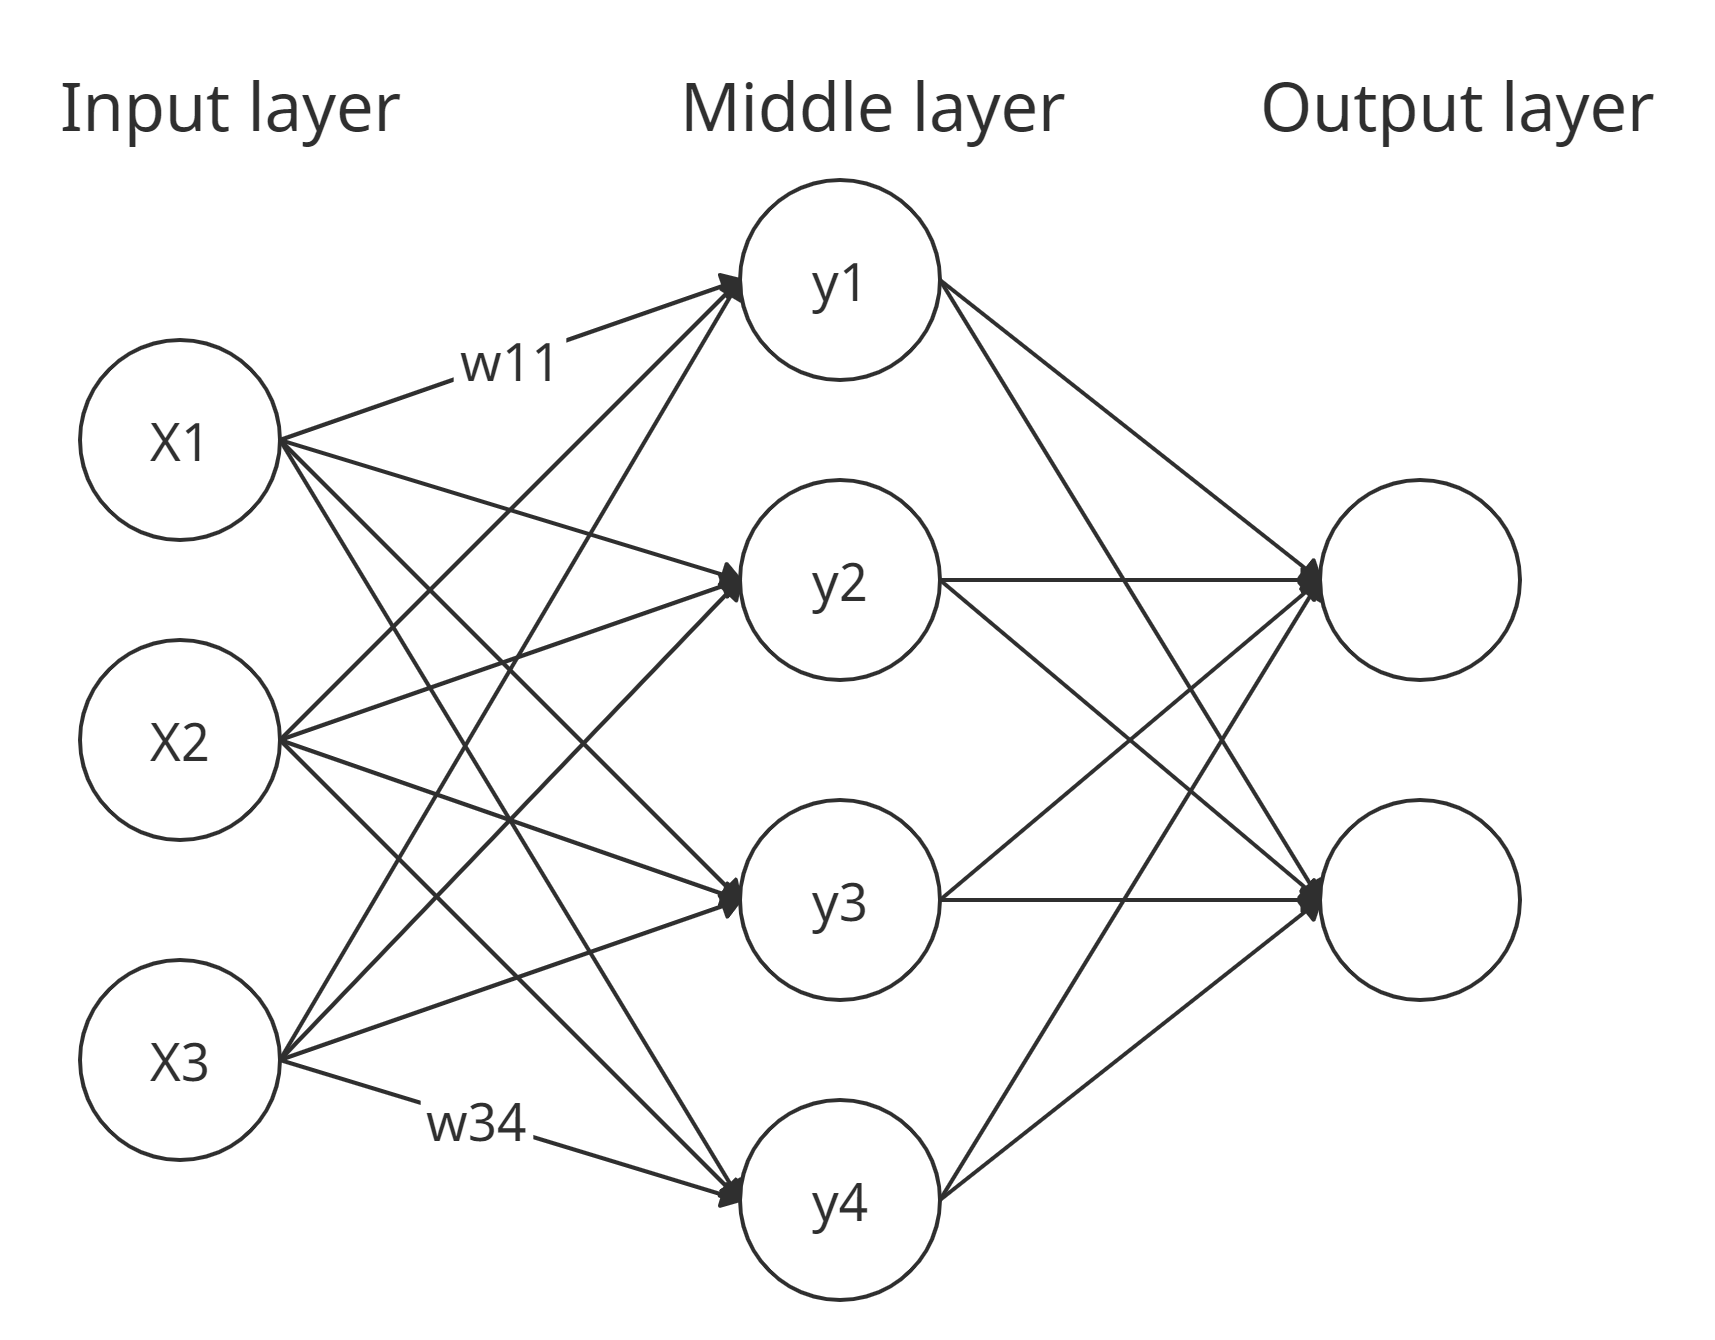
\includegraphics[width=7cm]{assets/images/FFN}
\caption{Architecture of a feedforward neural network
\label{fig:FFN}}
\end{figure}
\\At each layer a calculation is performed, which involves computing a weighted sum of the neuron's input values, followed by a functional operation. Performing this operation equals to applying a nonlinear activation function to the previously computed weighted sum \cite{tutorialIEEE}. The following formula is used at each layer:
\begin{equation}
    y_{j}=f\left({\sum \limits _{i=1}^{n} w_{ij} \times x_{i} + b}\right)
\end{equation}
where $y_j$ is the input value for j-th neuron in corresponding - in this case the middle - layer, $w$ are the weights, $x$ is the value of a neuron from previous layer, $b$ is the bias term and $f$ is the activation function, same as with perceptron mentioned earlier \cite{tutorialIEEE}. The number of neurons in the previous layer is in this case $n$.
\subsection{Deep neural networks}
In the deep networks domain, deep neural networks introduce the use of deep learning on a neural network model.
\begin{figure}[!ht]
\centering
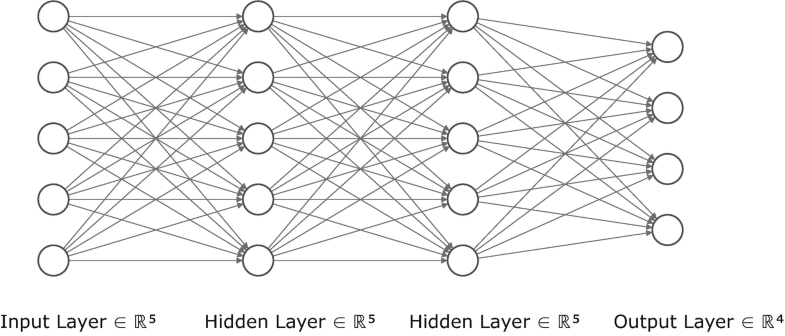
\includegraphics[width=12cm]{assets/images/DNN}
\caption{Architecture of a deep neural network with two hidden layers \footfullcite{chapterBookDL}
\label{fig:DNN}}
\end{figure}

\subsubsection{Activation functions}
\subsubsection*{Rectified linear function}
\subsubsection*{Sigmoid function}
\subsubsection{Gradient-based learning}
An optimization technique is what powers the deep learning process. Stochastic gradient descent is probably the most popular algorithm used for optimization. It is based on the simpler Gradient descent algorithm.
\subsubsection*{Gradient descent}
This algorithm uses the first derivative to find a global minimum of a function and thus provide optimization \cite{deeplearningbook}. Computing the derivative gives the answer to the question of how the model should adjust its parameters in order to improve its predictions.

\subsubsection*{Stochastic gradient descent}
% \begin{enumerate}[label={\arabic*.}]
% \vspace{-0.2cm}\item First Line
% \vspace{-0.4cm}\item Second Line 
% \end{enumerate}
\subsection{Convolutional neural networks}
% https://downloads.hindawi.com/journals/cin/2018/7068349.pdf

https://www2.cs.duke.edu/courses/spring19/compsci527/papers/Lecun.pdf
\section{Interpretability and explainability of neural networks}
\subsection{Layer-Wise Relevance Propagation}
\section{Challenges of deep learning}